\documentclass[11pt,a4paper]{article}
\usepackage[margin=2.2cm]{geometry}
\usepackage{amsmath,amssymb,mathtools,bm}
\usepackage{booktabs}
\usepackage{tikz}
\usetikzlibrary{arrows.meta,positioning,calc}
\usepackage[colorlinks=true,linkcolor=blue!50!black]{hyperref}
\numberwithin{equation}{section}
\setlength{\parindent}{0pt}
\setlength{\parskip}{4pt}

\newcommand{\cj}[1]{\overline{#1}}
\newcommand{\re}{\operatorname{Re}}
\newcommand{\im}{\operatorname{Im}}
\newcommand{\sat}{\operatorname{sat}}
\newcommand{\dd}{\mathrm{d}}
\newcommand{\blk}[1]{\textsf{#1}}

\title{Two-Machine Power System with a Grid-Forming Converter\\[2pt]
\large Governing Equations and Their Derivation, in the Order of the Simulink Models (Cases 1--4)}
\author{}
\date{}

\begin{document}
\maketitle
\noindent The test system, operating point and parameters are those of \cite{RA2021access,RA2023chapter}; the modelling follows \cite{Kundur1994,SauerPai1998}.

\paragraph{Study cases.} The equations below are those of the complete model \texttt{case3\_primary\_AGC\_GFM.slx}. The other cases are separate model files from which blocks are removed:
\begin{center}
\begin{tabular}{llccc}
\toprule
Case & Model file & AGC & GFM & States\\
\midrule
1 & \texttt{case1\_primary\_control.slx} & -- & -- & 18\\
2 & \texttt{case2\_primary\_AGC.slx} & \checkmark & -- & 20\\
3 & \texttt{case3\_primary\_AGC\_GFM.slx} & \checkmark & \checkmark & 23\\
4 & Case 3 model run with $K_i = 0$ & (off) & \checkmark & 23\\
\bottomrule
\end{tabular}
\end{center}
Study A compares Cases 1 and 2, Study B Cases 2 and 3, Study C Cases 1 and 4. Primary control (governor droop) is active in every case. The indicators $\gamma_{\text{agc}}$ (AGC present) and $\gamma_g$ (GFM present) used below are therefore not switches inside one model: they mark which equations exist in each case (Case 1: $\gamma_{\text{agc}}=\gamma_g=0$; Case 2: $\gamma_{\text{agc}}=1,\ \gamma_g=0$; Case 3: $\gamma_{\text{agc}}=\gamma_g=1$; Case 4: $\gamma_g=1$ with $K_i=0$). Bus 5 (the GFM connection point) and its transformer $x_{T5}$ exist only in the GFM model; Cases 1 and 2 use the 4-bus network of buses 1--4 (Section~\ref{sec:4bus}).


%======================================================================
\section{Base quantities, frames and per-unit conventions}
%
\noindent Per-unit system and phasor representation: \cite[Ch.~3]{Kundur1994}, \cite[Ch.~3]{SauerPai1998}.
%======================================================================

\subsection{Bases}
\begin{align}
S_{\text{base}} &= 100~\text{MVA}, \qquad f_0 = 50~\text{Hz}, \qquad \omega_s = 2\pi f_0~\text{rad/s},\\
k_{S1} &= \frac{S_1}{S_{\text{base}}},\qquad k_{S2} = \frac{S_2}{S_{\text{base}}},\qquad k_{Sg} = \frac{S_g}{S_{\text{base}}}.
\end{align}

\subsection{Change of power base}
A power $P$ [MW] expressed on two bases:
\begin{equation}
P = p^{(100)}\,S_{\text{base}} = p^{(\text{own})}\,S_i
\;\;\Longrightarrow\;\;
p^{(\text{own})} = \frac{p^{(100)}}{k_{Si}} .
\end{equation}
This is the gain \blk{to own base} $=1/k_{Si}$ used in every source block.

\subsection{Change of impedance base}
With equal voltage bases, $Z_{\text{base}} = V_{\text{base}}^2/S$, so
\begin{equation}
x^{(100)} = x^{(\text{own})}\,\frac{S_{\text{base}}}{S_i}
\;\;\Longrightarrow\;\;
x_{q1} = \frac{x_q}{k_{S1}},\qquad x_{q2} = \frac{x_q}{k_{S2}},\qquad x_g = \frac{0.15}{k_{Sg}} .
\end{equation}

Current base $I_b = S/V_b$, so a current changes base inversely to the impedance:
\begin{equation}
i^{(\text{own})} = \frac{i^{(100)}}{k_{Si}}\qquad(\text{gain \blk{Id to own base}} = 1/k_{Si}),
\qquad x^{(100)}i^{(100)} = x^{(\text{own})}i^{(\text{own})}.
\end{equation}

\subsection{Phasor (RMS) frame}
Every voltage is written as
\begin{equation}
v(t) = \sqrt{2}\,|V|\cos\!\big(\omega_s t + \theta(t)\big)
\;\;\longleftrightarrow\;\;
V = |V|e^{j\theta},
\end{equation}
i.e.\ all angles ($\delta_1,\delta_2,\delta_g,\theta_k$) are measured in a reference frame rotating at the synchronous speed $\omega_s$.
The instantaneous angular frequency of a phasor is
\begin{equation}
\omega(t) = \frac{\dd}{\dd t}\big(\omega_s t + \theta\big) = \omega_s + \dot\theta
\;\;\Longrightarrow\;\;
\omega^{\text{pu}} = 1 + \frac{\dot\theta}{\omega_s},
\qquad
\dot\theta = \omega_s\big(\omega^{\text{pu}} - 1\big).
\label{eq:angle-freq}
\end{equation}
Equation~\eqref{eq:angle-freq} is used three times in the model: for the rotor angle of each SG, for the GFM angle, and (inverted) for the bus-5 frequency measurement.

\subsection{Complex power}
For a current $I$ leaving a node of voltage $V$,
\begin{equation}
S = P + jQ = V\,\cj{I}.
\end{equation}

%======================================================================
\section{Model workspace: network data, load flow and initialisation}
%======================================================================

\subsection{Branch data}
\begin{center}
\begin{tabular}{ccl}
\toprule
Branch & $x$ [pu, 100 MVA] & Element\\
\midrule
1--2 & $x_{T1}=0.01$ & transformer of SG1\\
5--2 & $x_{T5}=0.01$ & transformer of GFM (Cases 3, 4 only)\\
3--4 & $x_{T2}=0.003$ & transformer of SG2\\
2--3 & $x_L = 0.2/2 = 0.1$ & two parallel tie-lines\\
\bottomrule
\end{tabular}
\end{center}
Two equal lines in parallel: $y_L = \frac{1}{j0.2}+\frac{1}{j0.2} = \frac{1}{j0.1}$, hence $x_L = 0.2/2$.
The equations below are written for the 5-bus network of the GFM model; the 4-bus network of Cases 1 and 2 is given in Section~\ref{sec:4bus}.

\subsection{Bus admittance matrix}
Formulation: \cite{BergenVittal2000}.
Kirchhoff's current law at bus $i$ with a series branch $i$--$j$ of admittance $y_{ij}=1/(jx_{ij})$:
\begin{equation}
I_i = \sum_{j} y_{ij}\,(V_i - V_j)
= \Big(\sum_j y_{ij}\Big)V_i - \sum_j y_{ij} V_j .
\end{equation}
Each branch therefore adds the stamp
\begin{equation}
\begin{bmatrix} Y_{ii} & Y_{ij}\\ Y_{ji} & Y_{jj}\end{bmatrix}
\;\mathrel{+}=\;
\begin{bmatrix} y_{ij} & -y_{ij}\\ -y_{ij} & y_{ij}\end{bmatrix},
\qquad
\bm I = \bm Y_{\text{bus}}\,\bm V,\quad \bm Y_{\text{bus}}\in\mathbb C^{5\times 5}.
\end{equation}

\subsection{Load-flow equations}
Newton--Raphson power flow: \cite{TinneyHart1967}, \cite{BergenVittal2000}, \cite{KothariNagrath2011}.
Injected complex power at every bus:
\begin{equation}
S_i = V_i\,\cj{I_i} = V_i\,\cj{\textstyle\sum_{k=1}^{5} Y_{ik}V_k},
\qquad
\bm S = \bm V \circ \cj{\bm Y_{\text{bus}}\bm V}.
\end{equation}
In polar form, with $Y_{ik}=G_{ik}+jB_{ik}$ and $\theta_{ik}=\theta_i-\theta_k$:
\begin{align}
P_i &= \sum_{k} |V_i||V_k|\big(G_{ik}\cos\theta_{ik} + B_{ik}\sin\theta_{ik}\big),\\
Q_i &= \sum_{k} |V_i||V_k|\big(G_{ik}\sin\theta_{ik} - B_{ik}\cos\theta_{ik}\big).
\end{align}
Bus types: bus 4 slack ($|V_4|=1,\ \theta_4=0$), bus 1 PV ($P_1=P_{SG1},\ |V_1|=1$), buses 2, 3, 5 PQ.
Unknowns and specified values:
\begin{align}
\bm z &= [\theta_1,\ \theta_2,\ \theta_3,\ \theta_5,\ |V_2|,\ |V_3|,\ |V_5|]^{\mathsf T},\\
\bm s &= \frac{1}{S_{\text{base}}}\,[P_{SG1},\ -P_{L2},\ -P_{L3},\ P_{GFM},\ 0,\ 0,\ Q_{GFM}]^{\mathsf T},\\
\bm g(\bm z) &= \big[P_1,\,P_2,\,P_3,\,P_5,\,Q_2,\,Q_3,\,Q_5\big]^{\mathsf T}(\bm z) - \bm s = \bm 0 .
\end{align}
Newton--Raphson: first-order Taylor expansion $\bm g(\bm z+\Delta\bm z)\approx \bm g(\bm z)+\bm J\Delta\bm z = \bm 0$ gives
\begin{equation}
\bm z^{(n+1)} = \bm z^{(n)} - \bm J^{-1}\bm g(\bm z^{(n)}),
\qquad
J_{:,k} \approx \frac{\bm g(\bm z + h\bm e_k) - \bm g(\bm z)}{h},\quad h=10^{-7}.
\end{equation}
Result: $\bm V^0$ (bus voltages) and $\bm S^0 = \bm V^0\circ\cj{\bm Y_{\text{bus}}\bm V^0}$ (bus injections).

\subsection{Network of the cases without the GFM (Cases 1 and 2)}\label{sec:4bus}
Without the GFM, bus 5 would be an open-ended bus behind $x_{T5}$ with no injection, so its branch would carry no current and $V_5 = V_2$; it is therefore removed and the network has buses 1--4 only:
\begin{equation}
\text{branches } \{1\text{--}2,\ 3\text{--}4,\ 2\text{--}3\},\qquad \bm Y_{\text{bus}}\in\mathbb C^{4\times 4},
\end{equation}
\begin{align}
\bm z &= [\theta_1,\ \theta_2,\ \theta_3,\ |V_2|,\ |V_3|]^{\mathsf T},\qquad
\bm s = \frac{1}{S_{\text{base}}}\,[P_{SG1},\ -P_{L2},\ -P_{L3},\ 0,\ 0]^{\mathsf T},\\
\bm g(\bm z) &= \big[P_1,\,P_2,\,P_3,\,Q_2,\,Q_3\big]^{\mathsf T}(\bm z) - \bm s = \bm 0,
\end{align}
with bus 4 slack and bus 1 PV as before. Removing the current-free bus 5 does not change the operating point or the dynamic response of buses 1--4.

\subsection{Machine (d,q) axes}\label{sec:dq}
The $q$-axis of a machine lies along the rotor angle $\delta$, the $d$-axis lags it by $90^\circ$ ($e^{j(\delta-\pi/2)}$). Projection of any network phasor $X$ on these axes:
\begin{equation}
X = (X_d + jX_q)\,e^{j(\delta-\pi/2)}
\;\;\Longrightarrow\;\;
X_d + jX_q = X\,e^{-j(\delta-\pi/2)} = jX\,e^{-j\delta}.
\label{eq:dq}
\end{equation}

\subsection{Stator equations of model 1.0}\label{sec:stator}
Park's transformation \cite{Park1929}; one-axis (flux-decay) model \cite{SauerPai1998}, \cite{Kundur1994}; the designation ``model 1.0'' (one $d$-axis and no $q$-axis rotor circuit) follows \cite{IEEE1110}. The full machine data are those of the GENROU model in \cite{RA2021access}, \cite{Pourbeik2016}.
Park's stator equations with $R_s=0$, stator transients neglected and $\omega\approx 1$ in the EMF terms:
\begin{equation}
V_d = -\psi_q,\qquad V_q = \psi_d .
\end{equation}
$q$-axis: no rotor circuit in model 1.0, so $\psi_q = -x_q I_q$. $d$-axis: field winding only,
\begin{align}
\psi_d &= -x_d I_d + x_{md} i_{fd},\qquad \psi_{fd} = -x_{md} I_d + x_{fd} i_{fd} .
\end{align}
Eliminating $i_{fd}$ with $i_{fd} = (\psi_{fd} + x_{md}I_d)/x_{fd}$:
\begin{equation}
\psi_d = -\Big(x_d - \frac{x_{md}^2}{x_{fd}}\Big)I_d + \frac{x_{md}}{x_{fd}}\psi_{fd}
= -x'_d I_d + E'_q,
\qquad x'_d \triangleq x_d - \frac{x_{md}^2}{x_{fd}},\quad E'_q \triangleq \frac{x_{md}}{x_{fd}}\psi_{fd}.
\end{equation}
Hence
\begin{equation}
\boxed{V_d = x_q I_q,\qquad V_q = E'_q - x'_d I_d .}
\label{eq:stator}
\end{equation}

\subsection{Voltage behind $x_q$ ($E_Q$)}
Define the phasor $\bar E_Q = V + jx_q I$. In $(d,q)$ coordinates, using \eqref{eq:dq}:
\begin{equation}
j\bar E_Q e^{-j\delta} = (V_d + jV_q) + jx_q(I_d + jI_q) = (V_d - x_qI_q) + j(V_q + x_qI_d).
\end{equation}
By \eqref{eq:stator} the real part is zero, so $\bar E_Q$ lies exactly on the $q$-axis:
\begin{equation}
\boxed{\bar E_Q = E_Q\,e^{j\delta},\qquad E_Q = V_q + x_qI_d = E'_q + (x_q - x'_d)\,I_d .}
\label{eq:EQ}
\end{equation}
This is why the network can treat each SG as a (time-varying) voltage $E_Q e^{j\delta}$ behind the constant reactance $x_q$.

\subsection{Initial values of the synchronous generators}
From the load-flow solution:
\begin{align}
I_1 &= \cj{(S_1^0/V_1^0)}, & \bar E_{Q1} &= V_1^0 + jx_{q1}I_1, & \delta_1^0 &= \arg\bar E_{Q1},\\
I_2 &= \cj{(S_4^0/V_4^0)}, & \bar E_{Q2} &= V_4^0 + jx_{q2}I_2, & \delta_2^0 &= \arg\bar E_{Q2}.
\end{align}
$d$-axis current on own base (Section~\ref{sec:dq} with $I/k_{Si}$):
\begin{equation}
I_{di}^0 = \re\Big\{ j\,\frac{I_i}{k_{Si}}\,e^{-j\delta_i^0}\Big\}.
\end{equation}
Transient EMF from \eqref{eq:EQ}, field voltage from $\dot E'_q = 0$ in \eqref{eq:field} (Section~\ref{sec:field}):
\begin{equation}
E'^{\,0}_{qi} = |\bar E_{Qi}| - (x_q - x'_d)\,I_{di}^0,\qquad
E_{fdi}^0 = E'^{\,0}_{qi} + (x_d - x'_d)\,I_{di}^0 .
\end{equation}
Exciter reference from the steady state of the exciter, $E_{fd} = K_A(V_{\text{ref}} - V_t)$:
\begin{equation}
V_{ti}^0 = |V_{k_i}^0|,\qquad V_{\text{ref},i} = V_{ti}^0 + \frac{E_{fdi}^0}{K_A}.
\end{equation}

\subsection{Initial value of the GFM}
\begin{equation}
E_g = V_5^0 + jx_g\,\cj{(S_5^0/V_5^0)},\qquad |E_g| = E_{g,\text{mag}}\ (\text{held fixed}),\qquad \delta_g^0 = \arg E_g .
\end{equation}
Mechanical, governor and GFM set-points on own base:
\begin{equation}
P_{m1}^0 = \frac{\re S_1^0}{k_{S1}},\qquad
P_{m2}^0 = \frac{\re S_4^0}{k_{S2}},\qquad
P_{g,\text{ref}} = \frac{\re S_5^0}{k_{Sg}},\qquad
\theta_5^0 = \arg V_5^0,
\end{equation}
\begin{equation}
P_{\text{tie}}^0 = \re\!\left\{V_2^0\,\cj{\left(\frac{V_2^0-V_3^0}{jx_L}\right)}\right\}.
\end{equation}

\subsection{Constant-impedance loads}
A load consuming $S_L$ at voltage $V$ represented by a shunt admittance $y_L$:
\begin{equation}
S_L = V\,\cj{(y_L V)} = \cj{y_L}\,|V|^2
\;\;\Longrightarrow\;\;
y_L = \frac{\cj{S_L}}{|V|^2}.
\end{equation}
Since the injection at a load bus is $S_i^0 = -S_{L,i}$:
\begin{equation}
y_{L2} = \frac{\cj{(-S_2^0)}}{|V_2^0|^2},\qquad
y_{L3} = \frac{\cj{(-S_3^0)}}{|V_3^0|^2}.
\end{equation}
Consequence: the actual load power is voltage dependent, $P_{Li}(t) = G_{Li}\,|V_i(t)|^2$.

\subsection{Norton equivalent of the sources (SGs and GFM)}
Every source is a voltage behind a reactance: SG$i$ is $\bar E_{Qi}$ behind $jx_{qi}$ at bus $k_i$ ($k_1=1$, $k_2=4$), the GFM is $E_g$ behind $jx_g$ at bus 5. For a source $E$ behind $jx$ connected to bus $k$:
\begin{equation}
I_{\text{out}} = \frac{E - V_k}{jx} = \underbrace{\frac{E}{jx}}_{\text{current source } J}\; - \;\underbrace{\frac{1}{jx}}_{\text{shunt}}\,V_k .
\end{equation}
The shunt part is moved into the admittance matrix, the current source becomes the injection. The GFM is treated exactly like the two SGs:
\begin{equation}
J_1 = \frac{\bar E_{Q1}}{jx_{q1}},\qquad J_2 = \frac{\bar E_{Q2}}{jx_{q2}},\qquad J_g = \frac{E_g}{jx_g}.
\end{equation}

\subsection{Augmented admittance matrix and impedance matrix}
\begin{align}
\bm Y_{\text{aug}} &= \bm Y_{\text{bus}} + \operatorname{diag}(0,\,y_{L2},\,y_{L3},\,0,\,0),\\
Y_{\text{aug},11} &\mathrel{+}= \frac{1}{jx_{q1}},\qquad Y_{\text{aug},44} \mathrel{+}= \frac{1}{jx_{q2}},\qquad Y_{\text{aug},55} \mathrel{+}= \frac{\gamma_g}{jx_g} .
\end{align}
Nodal equation with current-source injections only at buses 1, 4, 5:
\begin{equation}
\bm Y_{\text{aug}}\bm V = \bm e_1 J_1 + \bm e_4 J_2 + \bm e_5 J_g
\;\;\Longrightarrow\;\;
\bm V = \bm Z\,(\bm e_1 J_1 + \bm e_4 J_2 + \bm e_5 J_g),\qquad \bm Z = \bm Y_{\text{aug}}^{-1}.
\end{equation}
Keeping only the columns of the injected buses:
\begin{equation}
\boxed{\bm V = \bm Z_n \begin{bmatrix} J_1\\ J_2\\ J_g\end{bmatrix},\qquad
\bm Z_n = \bm Z_{:,[1,4,5]}\in\mathbb C^{5\times 3}\quad(\text{Case 3}).}
\end{equation}
In Cases 1 and 2 (4-bus network, no GFM): $\bm Y_{\text{aug}} = \bm Y_{\text{bus}} + \operatorname{diag}(0,y_{L2},y_{L3},0)$ with the two SG shunts, $\bm Z_n = \bm Z_{:,[1,4]}\in\mathbb C^{4\times 2}$ and $\bm V = \bm Z_n[J_1;\,J_2]$.

\subsection{Load step as a change of the impedance matrix}
A step $\Delta P_{L2}$ (\texttt{dP\_L2\_MW}) at bus 2 is a conductance change at nominal voltage:
\begin{equation}
\Delta G_{L2} = \frac{\Delta P_{L2}/S_{\text{base}}}{|V_2^0|^2},
\qquad
Y_{\text{aug},22}^{\text{post}} = Y_{\text{aug},22}^{\text{pre}} + \Delta G_{L2},
\end{equation}
\begin{equation}
\bm Z^{\text{post}} = \big(\bm Y_{\text{aug}}^{\text{post}}\big)^{-1},\qquad
\bm Z_n^{\text{post}} = \bm Z^{\text{post}}_{:,[1,4,5]}.
\end{equation}
With $\Delta P_{L2}=-100$ MW this is a load rejection in Area 1.

\subsection{Consistency check at $t=0$}
The model checks
\begin{equation}
\bm Z_n^{\text{pre}}\begin{bmatrix} \bar E_{Q1}/(jx_{q1})\\ \bar E_{Q2}/(jx_{q2})\\ E_g/(jx_g)\end{bmatrix} = \bm V^0 .
\end{equation}
At the operating point $P_{GFM}=Q_{GFM}=0$, so from the GFM initialisation $E_g = V_5^0$. The Norton source current and the current drawn by the shunt $1/(jx_g)$ then cancel,
\begin{equation}
I_g^0 = J_g^0 - \frac{V_5^0}{jx_g} = \frac{E_g - V_5^0}{jx_g} = 0,
\end{equation}
so adding the GFM does not disturb the load flow: its net contribution at $t=0$ is zero.

%======================================================================
\section{Network block (algebraic equations)}
%======================================================================
Inputs: $\delta_1,\ \delta_2,\ \delta_g,\ u_{\text{step}},\ E_{Q1},\ E_{Q2}$.
Outputs: $P_{e1}, P_{e2}, P_g, Q_g, \theta_5, |\bm V|, P_{\text{tie}}, Q_{e1}, Q_{e2}, I_{d1}, I_{d2}, V_{t1}, V_{t2}$.

\subsection{Source voltages (\blk{Source voltages})}
SG voltages from \eqref{eq:EQ}: magnitude $E_{Qi}$ comes from the field-winding block (time varying), angle from the swing equation. GFM: fixed magnitude, controlled angle.
\begin{equation}
E_1 = E_{Q1}\,e^{j\delta_1},\qquad
E_2 = E_{Q2}\,e^{j\delta_2},\qquad
E_g = |E_g|\,e^{j\delta_g}.
\end{equation}

\subsection{Network solution (\blk{Network solution})}\label{sec:network-solution}
\paragraph{Step 1: impedance selection by the load step.}
The step signal $u_{\text{step}}(t) = 0$ for $t<t_{\text{step}}$, $1$ for $t\ge t_{\text{step}}$ drives a switch (\blk{Select Zn}, threshold 0.5):
\begin{equation}
\bm Z_n(t) = \begin{cases}\bm Z_n^{\text{pre}}, & u_{\text{step}}<0.5\\ \bm Z_n^{\text{post}}, & u_{\text{step}}\ge 0.5\end{cases}.
\end{equation}

\paragraph{Step 2: Norton currents of the sources.}
(Blocks \blk{Norton SG1 1 over jxq1}, \blk{Norton SG2 1 over jxq2}, \blk{Norton GFM 1 over jxg}.)
\begin{equation}
J_1 = \frac{E_1}{jx_{q1}},\qquad J_2 = \frac{E_2}{jx_{q2}},\qquad J_g = \frac{E_g}{jx_g}.
\end{equation}

\paragraph{Step 3: all bus voltages.}
\begin{equation}
\boxed{\bm V = \bm Z_n\begin{bmatrix}J_1\\ J_2\\ J_g\end{bmatrix}
= \bm Z_{:,1}\frac{E_1}{jx_{q1}} + \bm Z_{:,4}\frac{E_2}{jx_{q2}} + \bm Z_{:,5}\frac{E_g}{jx_g} .}
\end{equation}

\paragraph{Step 4: GFM output current.}
The current that the GFM delivers to bus 5 is the Norton source current minus the current through its own shunt (blocks \blk{V bus 5}, \blk{Eg - V5}, \blk{GFM current 1 over jxg}):
\begin{equation}
\boxed{I_g = J_g - \frac{V_5}{jx_g} = \frac{E_g - V_5}{jx_g}.}
\end{equation}

\paragraph{Equivalence with the Thevenin form.}
Let $\bm Y_0 = \bm Y_{\text{aug}} - \tfrac{1}{jx_g}\bm e_5\bm e_5^{\mathsf T}$ be the network without the GFM, $\bm Z^{(0)} = \bm Y_0^{-1}$. Substituting $J_g = I_g + V_5/(jx_g)$ in the nodal equation gives $\bm Y_0\bm V = \bm e_1J_1+\bm e_4J_2+\bm e_5I_g$, hence $V_5 = V_{th} + Z_{th}I_g$ with $V_{th} = Z^{(0)}_{51}J_1 + Z^{(0)}_{54}J_2$, $Z_{th} = Z^{(0)}_{55}$, and with $I_g = (E_g - V_5)/(jx_g)$:
\begin{equation}
I_g = \frac{E_g - V_{th}}{jx_g + Z_{th}} .
\end{equation}
The Norton form used in the model and this Thevenin form give identical $\bm V$ and $I_g$; the Norton form treats the GFM in the same way as the SGs.

\subsection{Source powers (\blk{Source powers})}
Terminal current, power and $d$-axis current of SG$i$ (terminal bus $k_1=1$, $k_2=4$):
\begin{align}
I_{t1} &= \frac{E_1 - V_1}{jx_{q1}}, & S_{e1} &= V_1\,\cj{I_{t1}}, & P_{e1}&=\re S_{e1}, & Q_{e1}&=\im S_{e1},\\
I_{t2} &= \frac{E_2 - V_4}{jx_{q2}}, & S_{e2} &= V_4\,\cj{I_{t2}}, & P_{e2}&=\re S_{e2}, & Q_{e2}&=\im S_{e2},\\
       &                           & S_{g} &= V_5\,\cj{I_g},    & P_{g}&=\re S_{g}, & Q_{g}&=\im S_{g}.
\end{align}
\paragraph{Rotation to machine axes.} From \eqref{eq:dq}, on 100 MVA:
\begin{equation}
\boxed{I_{di} + jI_{qi} = j\,I_{ti}\,e^{-j\delta_i},\qquad I_{di} = \re\{jI_{ti}e^{-j\delta_i}\}.}
\end{equation}
(Blocks: \blk{exp(-j delta)} $\to$ \blk{Rotate to machine axes} $\to$ \blk{times j} $\to$ \blk{Id = Re}.)
\paragraph{Terminal voltages for the exciters.}
\begin{equation}
V_{t1} = |V_1|,\qquad V_{t2} = |V_4| .
\end{equation}

\paragraph{Terminal power equals power at $\bar E_Q$ (lossless reactance).}
\begin{equation}
E\cj I - V\cj I = (E-V)\cj I = jx_q\,I\cj I = jx_q|I|^2
\;\;\Longrightarrow\;\;
\re\{E\cj I\} = \re\{V\cj I\},\qquad \im\{E\cj I\} = \im\{V\cj I\} + x_q|I|^2 .
\end{equation}
Hence $P_{e1}$, $P_{e2}$, $P_g$ computed at the terminals are the electrical powers that enter the swing equation and the GFM droop.

\paragraph{Explicit nonlinear form.}
For $\bar E_Q=E_Qe^{j\delta}$, $V=|V|e^{j\theta}$:
\begin{equation}
S = V\,\cj{\frac{\bar E_Q-V}{jx_q}}
= \frac{j\big(|V|E_Qe^{-j(\delta-\theta)}-|V|^2\big)}{x_q},
\end{equation}
\begin{equation}
\boxed{P_e = \frac{E_Q|V|}{x_q}\sin(\delta-\theta),\qquad
Q_e = \frac{E_Q|V|\cos(\delta-\theta) - |V|^2}{x_q}.}
\end{equation}
\paragraph{Same power in terms of $E'_q$ (transient saliency).}
With $V_d = |V|\sin(\delta-\theta)$, $V_q = |V|\cos(\delta-\theta)$ and \eqref{eq:stator}: $I_q = V_d/x_q$, $I_d = (E'_q - V_q)/x'_d$, so (own base)
\begin{equation}
P_e = V_dI_d + V_qI_q
= \frac{E'_q|V|}{x'_d}\sin(\delta-\theta) + \frac{|V|^2}{2}\Big(\frac{1}{x_q}-\frac{1}{x'_d}\Big)\sin 2(\delta-\theta).
\end{equation}
Substituting $E_Q = E'_q + (x_q-x'_d)I_d$ in the boxed $P_e$ gives the same result, i.e.\ the $E_Q$-behind-$x_q$ network model is exact for model 1.0.

\subsection{Bus quantities (\blk{Bus quantities})}
\paragraph{Voltage magnitudes.} $|V_k|$, $k=1,\dots,5$ ($k=1,\dots,4$ in Cases 1 and 2).

\paragraph{Tie-line power (both lines, bus 2 $\to$ 3).}
\begin{equation}
I_{\text{line}} = \frac{V_2 - V_3}{jx_L},\qquad
S_{\text{tie}} = V_2\,\cj{I_{\text{line}}},\qquad
\boxed{P_{\text{tie}} = \re S_{\text{tie}} = \frac{|V_2||V_3|}{x_L}\sin(\theta_2-\theta_3).}
\end{equation}
(Same steps as the two-bus element above with $E\to V_2$, $V\to V_3$ and $\re\{V_2\cj I\}=\re\{V_3\cj I\}$ for a lossless line.)

\paragraph{Continuous (unwrapped) angle of bus 5.}
$\arg(\cdot)$ is limited to $(-\pi,\pi]$; to obtain a continuous angle the voltage is first rotated into the SG1 rotor frame:
\begin{equation}
\boxed{\theta_5 = \delta_1 + \arg\!\big(V_5\,e^{-j\delta_1}\big).}
\end{equation}
Since $|\theta_5-\delta_1|<\pi$ always holds, $\theta_5$ is continuous even when $\delta_1$ drifts by several turns.

\subsection{Closed nonlinear form of the network (Kron-reduced)}
Network reduction to internal nodes: \cite{BergenVittal2000,SauerPai1998}.
Combining the above, all source currents are linear in the internal voltages,
\begin{equation}
\begin{bmatrix} I_{t1}\\ I_{t2}\\ I_g\end{bmatrix}
= \bm Y_{\text{red}}\begin{bmatrix} E_1\\ E_2\\ E_g\end{bmatrix},\qquad
\bm Y_{\text{red}} = \bm Y_d - \bm Y_d\,\tilde{\bm Z}_{[1,4,5],[1,4,5]}\,\bm Y_d,
\end{equation}
\begin{equation}
\bm Y_d = \operatorname{diag}\!\Big(\tfrac{1}{jx_{q1}},\tfrac{1}{jx_{q2}},\tfrac{1}{jx_g}\Big),\qquad
\tilde{\bm Z} = \bm Z = \bm Y_{\text{aug}}^{-1}\quad(x_g\text{ already in }\bm Y_{\text{aug}}).
\end{equation}
Derivation: $I_{t,i} = (E_i - V_{k_i})/(jx_i) = Y_{d,ii}E_i - Y_{d,ii}V_{k_i}$ and $V_{k_i} = \sum_m \tilde Z_{k_i k_m} Y_{d,mm}E_m$ (Step 3 above).
With $Y_{\text{red},ik} = G_{ik}+jB_{ik}$ and $\delta_{ik}=\delta_i-\delta_k$:
\begin{equation}
\boxed{P_{i}(\bm\delta,\bm E_Q) = \re\{E_i\cj{I_i}\} = \sum_{k\in\{1,2,g\}} |E_i||E_k|\big(G_{ik}\cos\delta_{ik} + B_{ik}\sin\delta_{ik}\big)}
\label{eq:Pred}
\end{equation}
with $|E_1| = E_{Q1}(t)$, $|E_2| = E_{Q2}(t)$, $|E_g|$ constant. This is the nonlinear coupling of the angle states and of the field states (through $E_{Qi}$) through the network; $G_{ik}\neq 0$ because the constant-impedance loads are absorbed in $\bm Y_{\text{red}}$. The matrices change at $t_{\text{step}}$ ($\bm Y_{\text{red}}^{\text{pre}}\to\bm Y_{\text{red}}^{\text{post}}$).

%======================================================================
\section{Synchronous generator blocks \blk{SG1} and \blk{SG2}}
%======================================================================
Both blocks are identical in structure; index $i\in\{1,2\}$, rating $S_i$, $k_{Si}$, $\delta_i^0$, $P_{mi}^0$, $E'^{\,0}_{qi}$, $V_{\text{ref},i}$.
Inputs: $P_{ei}$ [pu, 100 MVA], $\Delta P_{\text{ref},i}$ [pu own], $I_{di}$ [pu, 100 MVA], $V_{ti}$ [pu]. Outputs: $\delta_i$, $\omega_i$, $P_{mi}$, $E_{Qi}$.

\subsection{Field winding, model 1.0 (\blk{Field winding (model 1.0)})}\label{sec:field}
Derivation follows \cite[Ch.~3]{SauerPai1998}, \cite[Ch.~3]{Kundur1994}; model structure per \cite{IEEE1110}.
\paragraph{Field circuit (Faraday + Ohm), per unit with time in seconds.}
\begin{equation}
\frac{1}{\omega_b}\frac{\dd\psi_{fd}}{\dd t} = v_{fd} - r_{fd}\,i_{fd}.
\end{equation}
Multiply by $x_{md}/r_{fd}$ and use $E'_q = \frac{x_{md}}{x_{fd}}\psi_{fd}$:
\begin{equation}
\underbrace{\frac{x_{fd}}{\omega_b r_{fd}}}_{T'_{d0}}\frac{\dd E'_q}{\dd t}
= \underbrace{\frac{x_{md}}{r_{fd}}v_{fd}}_{E_{fd}} - \underbrace{x_{md}\,i_{fd}}_{E_q}.
\end{equation}
Open-circuit EMF $E_q$ from $i_{fd} = (\psi_{fd}+x_{md}I_d)/x_{fd}$:
\begin{equation}
E_q = x_{md}i_{fd} = E'_q + \frac{x_{md}^2}{x_{fd}}I_d = E'_q + (x_d - x'_d)I_d .
\end{equation}
Therefore, with $I_{di}^{\text{own}} = I_{di}/k_{Si}$ (gain \blk{Id to own base}):
\begin{equation}
\boxed{T'_{d0}\frac{\dd E'_{qi}}{\dd t} = E_{fdi} - E'_{qi} - (x_d - x'_d)\,I_{di}^{\text{own}},\qquad E'_{qi}(0) = E'^{\,0}_{qi},}
\label{eq:field}
\end{equation}
\begin{equation}
\boxed{E_{Qi} = E'_{qi} + (x_q - x'_d)\,I_{di}^{\text{own}}}\qquad\text{(\blk{Voltage behind Xq}, from \eqref{eq:EQ})}.
\end{equation}
(Blocks: \blk{Field balance} $\to$ \blk{1 over Td0p} $\to$ \blk{Transient emf Eqp} $\to$ \blk{Voltage behind Xq}.)

\subsection{Excitation system (\blk{Exciter (IEEE ST1)})}
Model ST1 of \cite{IEEE4215}, see also \cite[Ch.~8]{Kundur1994}; parameters from \cite[Table~6]{RA2021access}.
\paragraph{Voltage transducer.} First-order lag, state $v_{Ri}$:
\begin{equation}
\boxed{T_R\frac{\dd v_{Ri}}{\dd t} = V_{ti} - v_{Ri},\qquad v_{Ri}(0) = V_{ti}^0,}
\qquad \frac{V_{Ri}}{V_{ti}}(s) = \frac{1}{1+sT_R}.
\end{equation}
\paragraph{Voltage error.}
\begin{equation}
u_{Ei} = V_{\text{ref},i} - v_{Ri}.
\end{equation}
\paragraph{Transient gain reduction (lead--lag).} Required: $\dfrac{Y}{U}(s) = \dfrac{1+sT_C}{1+sT_B}$. Split into a direct and a lag part:
\begin{equation}
\frac{1+sT_C}{1+sT_B} = \frac{T_C}{T_B} + \frac{1-T_C/T_B}{1+sT_B}
\quad\Big(\text{check: } \tfrac{T_C}{T_B}(1+sT_B) + 1 - \tfrac{T_C}{T_B} = 1 + sT_C\Big).
\end{equation}
Realisation with one state $x_{LLi}$:
\begin{equation}
\boxed{T_B\frac{\dd x_{LLi}}{\dd t} = u_{Ei} - x_{LLi},\qquad
y_i = \frac{T_C}{T_B}u_{Ei} + \Big(1-\frac{T_C}{T_B}\Big)x_{LLi},\qquad x_{LLi}(0) = \frac{E_{fdi}^0}{K_A}.}
\end{equation}
\paragraph{Exciter gain and ceiling.}
\begin{equation}
\boxed{E_{fdi} = \sat_{[V_{R\min},\,V_{R\max}]}\big(K_A\,y_i\big).}
\end{equation}
\paragraph{Overall (linear range).}
\begin{equation}
E_{fdi}(s) = K_A\frac{1+sT_C}{1+sT_B}\Big(V_{\text{ref},i} - \frac{V_{ti}(s)}{1+sT_R}\Big).
\end{equation}
\paragraph{Steady state.} $v_{Ri}=V_{ti}$, $x_{LLi}=u_{Ei}$, $y_i=u_{Ei}$, so $E_{fdi} = K_A(V_{\text{ref},i}-V_{ti})$; with $V_{\text{ref},i} = V_{ti}^0 + E_{fdi}^0/K_A$ the initial state is an equilibrium.

\subsection{Swing equation (\blk{Swing equation})}
Derivation follows \cite[Ch.~3]{Kundur1994}, \cite[Ch.~3]{SauerPai1998}, \cite{KothariNagrath2011}.
\paragraph{Newton's second law for the rotor.}
\begin{equation}
J\frac{\dd\omega_{m}}{\dd t} = T_m - T_e - T_D .
\end{equation}
\paragraph{Inertia constant.}
\begin{equation}
H = \frac{\tfrac12 J\omega_{sm}^2}{S_i}\;[\text{s}]
\;\;\Longrightarrow\;\;
J = \frac{2HS_i}{\omega_{sm}^2}.
\end{equation}
\paragraph{Per-unit form.} Divide by the base torque $T_b = S_i/\omega_{sm}$ and write $\omega = \omega_m/\omega_{sm}$:
\begin{equation}
\frac{2HS_i}{\omega_{sm}^2}\,\omega_{sm}\frac{\dd\omega}{\dd t}\cdot\frac{\omega_{sm}}{S_i}
= T_m^{\text{pu}} - T_e^{\text{pu}} - T_D^{\text{pu}}
\;\;\Longrightarrow\;\;
2H\frac{\dd\omega}{\dd t} = T_m^{\text{pu}} - T_e^{\text{pu}} - T_D^{\text{pu}} .
\end{equation}
\paragraph{Power to torque.} $P = T\omega_m \Rightarrow T^{\text{pu}} = P^{\text{pu}}/\omega$. Damping $T_D^{\text{pu}} = D(\omega-1)$.
Electrical power converted to own base, $P_{ei}/k_{Si}$:
\begin{equation}
\boxed{\frac{\dd\omega_i}{\dd t} = \frac{1}{2H}\left[\frac{P_{mi} - P_{ei}/k_{Si}}{\omega_i} - D(\omega_i - 1)\right],\qquad \omega_i(0)=1.}
\label{eq:swing}
\end{equation}
(Blocks: \blk{to own base} $\to$ \blk{Accelerating power} $\to$ \blk{Torque} ($\div\omega$) $\to$ \blk{Minus damping} $\to$ \blk{1 over 2H} $\to$ \blk{Speed}.)

\paragraph{Rotor angle.} Electrical rotor angle relative to the synchronous frame, from \eqref{eq:angle-freq}:
\begin{equation}
\boxed{\frac{\dd\delta_i}{\dd t} = \omega_s(\omega_i - 1),\qquad \delta_i(0) = \delta_i^0.}
\label{eq:rotor-angle}
\end{equation}
(Blocks: \blk{Speed deviation} $\to$ \blk{omega\_s} $\to$ \blk{Rotor angle}.)

\paragraph{Second-order nonlinear form.} Substituting \eqref{eq:Pred} into \eqref{eq:swing}--\eqref{eq:rotor-angle}:
\begin{equation}
\frac{2H}{\omega_s}\,\ddot\delta_i
= \frac{P_{mi} - \tfrac{1}{k_{Si}}P_i(\delta_1,\delta_2,\delta_g,E_{Q1},E_{Q2})}{1+\dot\delta_i/\omega_s}
- \frac{D}{\omega_s}\dot\delta_i .
\end{equation}
Here $D=2$ represents the damper windings that model 1.0 omits.

\subsection{Speed governor (\blk{Governor (IEEEG1)})}
IEEEG1 governor \cite{IEEE1973,PESTR1}; parameters from \cite[Table~7]{RA2021access}; see also \cite[Ch.~9]{Kundur1994}.
\paragraph{Load reference.}
\begin{equation}
P_{\text{ref},i} = P_{mi}^0 + \Delta P_{\text{ref},i}\quad(\Delta P_{\text{ref},i}\text{ from the AGC}).
\end{equation}
\paragraph{Governor error (droop feedback and valve-position feedback).}
\begin{equation}
e_{gi} = P_{\text{ref},i} - K(\omega_i - 1) - g_{vi},\qquad K = \frac{1}{R} .
\end{equation}
\paragraph{Servo motor with rate limit.}
\begin{equation}
r_i = \sat_{[U_c,\,U_o]}\!\left(\frac{1}{T_3}\,e_{gi}\right),
\end{equation}
\paragraph{Valve position with position limits (limited integrator).}
\begin{equation}
\boxed{\frac{\dd g_{vi}}{\dd t} =
\begin{cases}
0, & g_{vi}=P_{\max}\ \text{and}\ r_i>0,\\
0, & g_{vi}=P_{\min}\ \text{and}\ r_i<0,\\
r_i, & \text{otherwise},
\end{cases}
\qquad g_{vi}(0)=P_{mi}^0 .}
\end{equation}
\paragraph{Linear range.} Without limits,
\begin{equation}
T_3\dot g_{vi} = P_{\text{ref},i} - K\Delta\omega_i - g_{vi}
\;\;\Longrightarrow\;\;
G_{vi}(s) = \frac{1}{1+sT_3}\big(P_{\text{ref},i}(s) - K\Delta\omega_i(s)\big).
\end{equation}
\paragraph{Droop.} In steady state $\dot g_{vi}=0$:
\begin{equation}
g_{vi} = P_{\text{ref},i} - K\Delta\omega_i
\;\;\Longrightarrow\;\;
R = -\frac{\Delta\omega_i}{\Delta g_{vi}} = \frac{1}{K} = 0.05~\text{pu}\;(5\,\%).
\end{equation}

\subsection{Reheat steam turbine (\blk{Turbine (reheat)})}
Tandem-compound single-reheat turbine \cite{IEEE1973,PESTR1}, \cite[Ch.~9]{Kundur1994}.
\paragraph{First-order lag of a steam volume.}
Mass in a volume $m$; outflow proportional to stored mass (pressure), $q_{\text{out}} = m/T$:
\begin{equation}
\frac{\dd m}{\dd t} = q_{\text{in}} - q_{\text{out}} = q_{\text{in}} - \frac{m}{T}
\;\;\Longrightarrow\;\;
T\frac{\dd q_{\text{out}}}{\dd t} = q_{\text{in}} - q_{\text{out}},
\qquad
\frac{q_{\text{out}}}{q_{\text{in}}}(s) = \frac{1}{1+sT}.
\end{equation}
Implemented in each sub-block as $\dot x = \frac{1}{T}(u - x)$ (\blk{Error} $\to$ \blk{One over T} $\to$ \blk{State}).

\paragraph{Steam chest, reheater, crossover in cascade.}
\begin{align}
\frac{\dd x_{HP,i}}{\dd t} &= \frac{1}{T_4}\big(g_{vi} - x_{HP,i}\big), & x_{HP,i}(0)&=P_{mi}^0,\\
\frac{\dd x_{IP,i}}{\dd t} &= \frac{1}{T_5}\big(x_{HP,i} - x_{IP,i}\big), & x_{IP,i}(0)&=P_{mi}^0,\\
\frac{\dd x_{LP,i}}{\dd t} &= \frac{1}{T_6}\big(x_{IP,i} - x_{LP,i}\big), & x_{LP,i}(0)&=P_{mi}^0.
\end{align}
\paragraph{Mechanical power.}
\begin{equation}
\boxed{P_{mi} = K_1 x_{HP,i} + K_3 x_{IP,i} + K_5 x_{LP,i},\qquad K_1+K_3+K_5 = 1.}
\end{equation}
\paragraph{Transfer function.}
\begin{equation}
\frac{P_{mi}}{G_{vi}}(s) = \frac{1}{1+sT_4}\left[K_1 + \frac{K_3}{1+sT_5} + \frac{K_5}{(1+sT_5)(1+sT_6)}\right],
\qquad
\left.\frac{P_{mi}}{G_{vi}}\right|_{s=0} = K_1+K_3+K_5 = 1 .
\end{equation}

\subsection{Interconnection inside an SG block}
\begin{align}
&\Delta P_{\text{ref},i}\;\xrightarrow{\text{governor}}\; g_{vi}\;\xrightarrow{\text{turbine}}\;P_{mi}\;\xrightarrow{\text{swing}}\;(\omega_i,\delta_i),
\qquad \omega_i\to\text{governor},\quad P_{ei}\to\text{swing},\\
&V_{ti}\;\xrightarrow{\text{exciter}}\;E_{fdi}\;\xrightarrow{\text{field winding}}\;E'_{qi}\;\to\;E_{Qi}\;\to\;\text{network},
\qquad I_{di}\to\text{field winding}.
\end{align}

%======================================================================
\section{Grid-forming converter block \blk{GFM}}
%
\noindent GFM with P--f droop and POD-P stabilizer as proposed in \cite{RA2021access,RA2023chapter}.
%======================================================================
Inputs: $P_g$ [pu, 100 MVA], $f_{\text{meas}}$ [pu]. Outputs: $\delta_g$, $\omega_g$.
The converter is an ideal voltage source $E_g = |E_g|e^{j\delta_g}$ (magnitude fixed) behind $x_g$; only its angle is controlled.

\subsection{Power error and P--f droop}
\begin{equation}
P_g^{\text{own}} = \frac{P_g}{k_{Sg}},\qquad
\Delta\omega_{\text{droop}} = R_g\big(P_{g,\text{ref}} - P_g^{\text{own}}\big).
\end{equation}
Derivation of the droop law: a synchronous machine in steady state follows $\Delta\omega = -R\,\Delta P$; the GFM imposes the same relation directly on its internal frequency, so that $P_g$ rises when frequency falls.

\subsection{Power-oscillation damper (POD-P) with washout}
Measured frequency deviation:
\begin{equation}
\Delta\omega_{\text{meas}} = f_{\text{meas}} - 1 .
\end{equation}
Washout realised with an integrator state $z$:
\begin{equation}
\boxed{\frac{\dd z}{\dd t} = \frac{\gamma_g}{T_w}\big(\Delta\omega_{\text{meas}} - z\big),\qquad z(0)=0,}
\end{equation}
\begin{equation}
w = \Delta\omega_{\text{meas}} - z,\qquad
\frac{Z(s)}{\Delta\Omega_{\text{meas}}(s)} = \frac{1}{1+sT_w}
\;\;\Longrightarrow\;\;
\frac{W(s)}{\Delta\Omega_{\text{meas}}(s)} = 1-\frac{1}{1+sT_w} = \frac{sT_w}{1+sT_w}.
\end{equation}
POD term: $u_{\text{POD}} = K_w\,\gamma_{\text{pod}}\,w$, $\gamma_{\text{pod}} = \texttt{pod\_on}$. The washout removes the steady-state component, so the POD acts only during transients.

\subsection{Internal frequency}
\begin{equation}
\boxed{\omega_g = 1 + R_g\big(P_{g,\text{ref}} - P_g/k_{Sg}\big) - K_w\gamma_{\text{pod}}\big(\Delta\omega_{\text{meas}} - z\big).}
\end{equation}
In Laplace form:
\begin{equation}
\Delta\Omega_g(s) = -R_g\,\Delta P_g^{\text{own}}(s) - K_w\gamma_{\text{pod}}\frac{sT_w}{1+sT_w}\,\Delta\Omega_{\text{meas}}(s).
\end{equation}

\subsection{Converter angle}
From \eqref{eq:angle-freq}:
\begin{equation}
\boxed{\frac{\dd\delta_g}{\dd t} = \gamma_g\,\omega_s(\omega_g - 1),\qquad \delta_g(0) = \delta_g^0.}
\end{equation}
\paragraph{Combined first-order nonlinear form.}
\begin{equation}
\frac{1}{\omega_s R_g}\,\dot\delta_g
= P_{g,\text{ref}} - \frac{1}{k_{Sg}}P_g(\delta_1,\delta_2,\delta_g) - \frac{K_w\gamma_{\text{pod}}}{R_g}\big(\Delta\omega_{\text{meas}}-z\big)\qquad(\gamma_g=1).
\end{equation}
Compared with the swing equation (second order, inertia $2H$), the droop GFM is first order: zero inertia and an equivalent damping coefficient $1/(\omega_sR_g)$.

\paragraph{Steady state.} With $\dot\delta_g = 0$ in a common frequency $\omega$ and $w=0$:
\begin{equation}
P_g^{\text{own}} = P_{g,\text{ref}} - \frac{\omega - 1}{R_g}
\;\;\Longrightarrow\;\;
\Delta P_g^{(100)} = -\frac{k_{Sg}}{R_g}\Delta\omega .
\label{eq:gfm-ss}
\end{equation}

%======================================================================
\section{Bus-5 frequency measurement (\blk{Bus 5 frequency measurement})}
%======================================================================
Ideal bus frequency from \eqref{eq:angle-freq}: $f_5 = 1 + \dot\theta_5/\omega_s$.
A pure derivative is not realisable, so it is filtered:
\begin{equation}
\widehat{\dot\theta_5}(s) = \frac{s}{1+sT_f}\,\theta_5(s).
\end{equation}
Realisation with a state $\hat\theta_5$ (\blk{Filtered angle}):
\begin{equation}
\boxed{\frac{\dd\hat\theta_5}{\dd t} = \frac{1}{T_f}\big(\theta_5 - \hat\theta_5\big),\qquad \hat\theta_5(0) = \theta_5^0,}
\end{equation}
since $\hat\theta_5 = \frac{1}{1+sT_f}\theta_5 \Rightarrow s\hat\theta_5 = \frac{s}{1+sT_f}\theta_5$. Output:
\begin{equation}
\boxed{f_{\text{meas}} = 1 + \frac{1}{\omega_s}\cdot\frac{\theta_5 - \hat\theta_5}{T_f}.}
\end{equation}
$\hat\theta_5(0)=\theta_5^0$ gives $f_{\text{meas}}(0)=1$ (no start-up transient).

%======================================================================
\section{Secondary control block \blk{Secondary control (AGC)}}
%
\noindent Tie-line bias control: \cite[Ch.~11]{Kundur1994}, \cite{KothariNagrath2011}, \cite{KulkarniNPTEL}.
%======================================================================
Inputs (via Goto/From): $\omega_1$, $\omega_2$, $P_{\text{tie}}$. Outputs: $\Delta P_{\text{ref},1}$, $\Delta P_{\text{ref},2}$.
Area 1 = SG1 (+ GFM), Area 2 = SG2.

\subsection{Area frequency deviations and tie-line deviation}
\begin{equation}
\Delta f_1 = \omega_1 - 1,\qquad \Delta f_2 = \omega_2 - 1,\qquad
\Delta P_{\text{tie}} = P_{\text{tie}} - P_{\text{tie}}^0 .
\end{equation}
For the lossless tie, the export of Area 2 is $\Delta P_{\text{tie},2} = -\Delta P_{\text{tie}}$.

\subsection{Frequency bias = area frequency response characteristic}
Static response of each area to a frequency change $\Delta f$ (on 100 MVA): from the governor droop, $\Delta P_{mi}^{(100)} = -k_{Si}K\Delta f$; from \eqref{eq:gfm-ss}, $\Delta P_g^{(100)} = -\frac{k_{Sg}}{R_g}\Delta f$. The loads are static (no load damping). The bias set in the AGC block uses the governor and GFM droops:
\begin{equation}
\boxed{B_1 = K\,k_{S1} + \gamma_g\frac{k_{Sg}}{R_g},\qquad B_2 = K\,k_{S2}\qquad[\text{pu}_{100}/\text{pu}_f].}
\end{equation}
The rotor damping $D$ adds a further static response: from \eqref{eq:swing} at $\dot\omega_i=0$, $P_{ei}/k_{Si} = P_{mi} - D\,\omega_i\Delta\omega_i \approx P_{mi} - D\Delta\omega_i$, i.e.\ $\Delta P_{ei}^{(100)} \approx \Delta P_{mi}^{(100)} - k_{Si}D\Delta f$. The true area frequency response characteristic is therefore
\begin{equation}
\beta_1 = (K+D)\,k_{S1} + \gamma_g\frac{k_{Sg}}{R_g},\qquad \beta_2 = (K+D)\,k_{S2},
\end{equation}
and $B_i = \beta_i - D\,k_{Si}$ (bias slightly below $\beta_i$).

\subsection{Area control errors}
\begin{equation}
\boxed{ACE_1 = \Delta P_{\text{tie}} + B_1\Delta f_1,\qquad ACE_2 = -\Delta P_{\text{tie}} + B_2\Delta f_2 .}
\end{equation}

\subsection{Integral control (set-point changes)}
Converted to the own base of each machine:
\begin{equation}
\boxed{\frac{\dd\,\Delta P_{\text{ref},1}}{\dd t} = -\gamma_{\text{agc}}\frac{K_i}{k_{S1}}\,ACE_1,\qquad
\frac{\dd\,\Delta P_{\text{ref},2}}{\dd t} = -\gamma_{\text{agc}}\frac{K_i}{k_{S2}}\,ACE_2,}
\end{equation}
$\Delta P_{\text{ref},i}(0)=0$; $\gamma_{\text{agc}}=1$ in Cases 2 and 3 (in Case 4 the same block runs with $K_i=0$), and the AGC block does not exist in Case 1.
\paragraph{Why integral control.} In equilibrium the integrator inputs are zero, so $ACE_1 = ACE_2 = 0$; this is proved in Section~\ref{sec:ss}.

%======================================================================
\section{Load step, scaling and logged outputs}
%======================================================================
\begin{align}
u_{\text{step}}(t) &= \begin{cases}0,& t<t_{\text{step}}\\1,& t\ge t_{\text{step}}\end{cases}
\quad(\text{size } \Delta P_{L2} \text{ is inside } \bm Z_n^{\text{post}}),\\
f_i\,[\text{Hz}] &= f_0\,\omega_i,\qquad f_{5}\,[\text{Hz}] = f_0\,f_{\text{meas}},\\
P_{ei}\,[\text{MW}] &= S_{\text{base}}P_{ei},\quad P_g\,[\text{MW}] = S_{\text{base}}P_g,\quad P_{\text{tie}}\,[\text{MW}] = S_{\text{base}}P_{\text{tie}},\\
P_{mi}\,[\text{MW}] &= S_i\,P_{mi},\qquad Q\,[\text{MVAr}] = S_{\text{base}}\,Q .
\end{align}

%======================================================================
\section{Complete nonlinear model and interconnection}
%======================================================================

\subsection{Signal flow of the top level}
\begin{center}
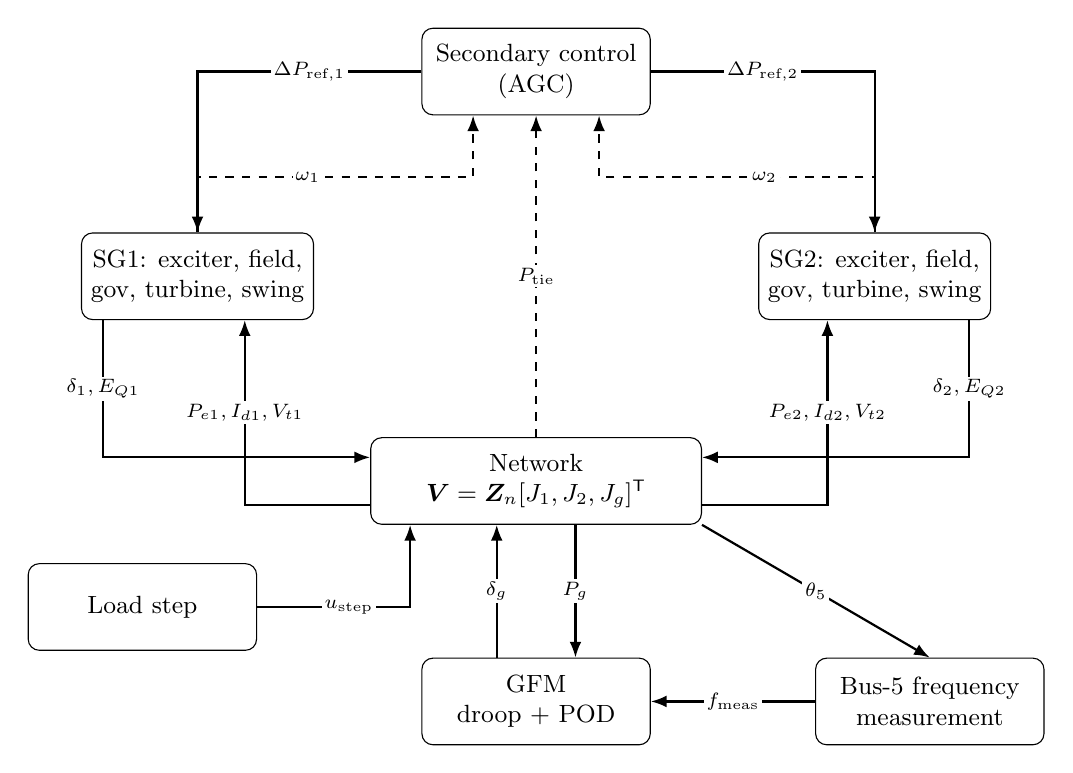
\begin{tikzpicture}[
  box/.style={draw,rounded corners,minimum width=2.9cm,minimum height=1.1cm,align=center,font=\small},
  ar/.style={-{Latex[length=2mm]},thick},
  lab/.style={font=\scriptsize,midway,fill=white,inner sep=1pt}]
\node[box] (agc) at (0,4.6) {Secondary control\\(AGC)};
\node[box] (sg1) at (-4.3,2) {SG1: exciter, field,\\gov, turbine, swing};
\node[box] (sg2) at (4.3,2) {SG2: exciter, field,\\gov, turbine, swing};
\node[box,minimum width=4.2cm] (net) at (0,-0.6) {Network\\$\bm V=\bm Z_n[J_1,J_2,J_g]^{\mathsf T}$};
\node[box] (gfm) at (0,-3.4) {GFM\\droop + POD};
\node[box] (fm) at (5,-3.4) {Bus-5 frequency\\measurement};
\node[box] (st) at (-5,-2.2) {Load step};
\draw[ar] (agc) -| node[lab,pos=0.25]{$\Delta P_{\text{ref},1}$} (sg1);
\draw[ar] (agc) -| node[lab,pos=0.25]{$\Delta P_{\text{ref},2}$} (sg2);
\draw[ar] ([xshift=-12mm]sg1.south) |- node[lab,pos=0.25]{$\delta_1,E_{Q1}$} ([yshift=3mm]net.west);
\draw[ar] ([yshift=-3mm]net.west) -| node[lab,pos=0.75]{$P_{e1},I_{d1},V_{t1}$} ([xshift=6mm]sg1.south);
\draw[ar] ([xshift=12mm]sg2.south) |- node[lab,pos=0.25]{$\delta_2,E_{Q2}$} ([yshift=3mm]net.east);
\draw[ar] ([yshift=-3mm]net.east) -| node[lab,pos=0.75]{$P_{e2},I_{d2},V_{t2}$} ([xshift=-6mm]sg2.south);
\draw[ar] ([xshift=-5mm]gfm.north) -- node[lab]{$\delta_g$} ([xshift=-5mm]net.south);
\draw[ar] ([xshift=5mm]net.south) -- node[lab]{$P_g$} ([xshift=5mm]gfm.north);
\draw[ar] (net.south east) -- node[lab]{$\theta_5$} (fm.north);
\draw[ar] (fm) -- node[lab]{$f_{\text{meas}}$} (gfm);
\draw[ar] (st.east) -| node[lab,pos=0.3]{$u_{\text{step}}$} ([xshift=-16mm]net.south);
\draw[ar,dashed] (sg1.north) -- ++(0,0.7) -| node[lab,pos=0.2]{$\omega_1$} ([xshift=-8mm]agc.south);
\draw[ar,dashed] (sg2.north) -- ++(0,0.7) -| node[lab,pos=0.2]{$\omega_2$} ([xshift=8mm]agc.south);
\draw[ar,dashed] (net.north) -- node[lab]{$P_{\text{tie}}$} (agc.south);
\end{tikzpicture}
\end{center}
Dashed lines are Goto/From connections; $I_{d1}$, $I_{d2}$, $V_{t1}$, $V_{t2}$ also reach the SG blocks through Goto/From. ($\delta_1,\delta_2$ are also used inside the network for $I_{d1}$, $I_{d2}$ and $\delta_1$ for the unwrapped angle $\theta_5$.)

\subsection{State vector (23 states in Case 3)}
\begin{align}
\bm x_{SGi} &= \big[\delta_i,\ \omega_i,\ E'_{qi},\ v_{Ri},\ x_{LLi},\ g_{vi},\ x_{HP,i},\ x_{IP,i},\ x_{LP,i}\big]^{\mathsf T},\qquad i=1,2,\\
\bm x &= \big[\bm x_{SG1}^{\mathsf T},\ \bm x_{SG2}^{\mathsf T},\ \underbrace{\delta_g,\ z}_{\text{GFM}},\ \underbrace{\hat\theta_5}_{\text{meas.}},\ \underbrace{\Delta P_{\text{ref},1},\ \Delta P_{\text{ref},2}}_{\text{AGC}}\big]^{\mathsf T}.
\end{align}
Case 2 has no GFM and no bus-5 frequency measurement (20 states); Case 1 has in addition no AGC (18 states).

\subsection{Differential--algebraic system}
Simultaneous solution of the machine differential equations and the algebraic network equations, as in the transient-stability procedure of \cite{KothariNagrath2011}, extended to the multimachine model of \cite{SauerPai1998}.
\paragraph{Algebraic equations (network, solved at every instant):}
\begin{align}
E_{Qi} &= E'_{qi} + (x_q-x'_d)\frac{I_{di}}{k_{Si}}\quad(i=1,2),\label{eq:alg-EQ}\\
E_1 &= E_{Q1}e^{j\delta_1},\quad E_2 = E_{Q2}e^{j\delta_2},\quad E_g = |E_g|e^{j\delta_g},\\
\bm V &= \bm Z_n\Big[\tfrac{E_1}{jx_{q1}},\ \tfrac{E_2}{jx_{q2}},\ \tfrac{E_g}{jx_g}\Big]^{\mathsf T},\qquad
I_g = \frac{E_g - V_5}{jx_g},\\
I_{t1} &= \tfrac{E_1-V_1}{jx_{q1}},\quad I_{t2} = \tfrac{E_2-V_4}{jx_{q2}},\quad
I_{di} = \re\{jI_{ti}e^{-j\delta_i}\},\quad V_{t1}=|V_1|,\ V_{t2}=|V_4|,\\
P_{e1} &= \re\{V_1\cj{I_{t1}}\},\quad
P_{e2} = \re\{V_4\cj{I_{t2}}\},\quad
P_g = \re\{V_5\cj{I_g}\},\\
P_{\text{tie}} &= \re\Big\{V_2\cj{\tfrac{V_2-V_3}{jx_L}}\Big\},\qquad
\theta_5 = \delta_1 + \arg(V_5e^{-j\delta_1}),\\
f_{\text{meas}} &= 1 + \frac{\theta_5-\hat\theta_5}{\omega_sT_f},\qquad
\omega_g = 1 + R_g\Big(P_{g,\text{ref}} - \tfrac{P_g}{k_{Sg}}\Big) - K_w\gamma_{\text{pod}}(f_{\text{meas}}-1-z),\\
u_{Ei} &= V_{\text{ref},i} - v_{Ri},\qquad E_{fdi} = \sat\Big(K_A\Big[\tfrac{T_C}{T_B}u_{Ei} + \big(1-\tfrac{T_C}{T_B}\big)x_{LLi}\Big]\Big),\\
e_{gi} &= P_{mi}^0 + \Delta P_{\text{ref},i} - K(\omega_i-1) - g_{vi},\qquad
P_{mi} = K_1x_{HP,i}+K_3x_{IP,i}+K_5x_{LP,i}.
\end{align}
\paragraph{Implicit loop $E_{Qi}\leftrightarrow I_{di}$.} \eqref{eq:alg-EQ} needs $I_{di}$, which depends on $E_{Q1},E_{Q2}$ through the network. Because the network is linear in $(E_{Q1},E_{Q2})$ for fixed angles,
\begin{equation}
I_{di} = \sum_{k=1,2} a_{ik}(\bm\delta,u_{\text{step}})\,E_{Qk} + b_i(\bm\delta,u_{\text{step}}),
\end{equation}
so \eqref{eq:alg-EQ} is a $2\times 2$ linear system for $E_{Q1},E_{Q2}$ at every instant; Simulink solves this algebraic loop numerically (\texttt{ode15s}, DAE index 1).
\paragraph{Differential equations ($i=1,2$):}
\begin{align}
\dot\delta_i &= \omega_s(\omega_i-1),\\
\dot\omega_i &= \frac{1}{2H}\Big[\frac{P_{mi}-P_{ei}/k_{Si}}{\omega_i} - D(\omega_i-1)\Big],\\
\dot E'_{qi} &= \frac{1}{T'_{d0}}\Big[E_{fdi} - E'_{qi} - (x_d-x'_d)\frac{I_{di}}{k_{Si}}\Big],\\
\dot v_{Ri} &= \frac{1}{T_R}(V_{ti} - v_{Ri}),\qquad
\dot x_{LLi} = \frac{1}{T_B}(u_{Ei} - x_{LLi}),\\
\dot g_{vi} &= \sat_{[U_c,U_o]}\Big(\frac{1}{T_3}e_{gi}\Big)\ \text{with } g_{vi}\in[P_{\min},P_{\max}],\\
\dot x_{HP,i} &= (g_{vi}-x_{HP,i})/T_4,\quad
\dot x_{IP,i} = (x_{HP,i}-x_{IP,i})/T_5,\quad
\dot x_{LP,i} = (x_{IP,i}-x_{LP,i})/T_6,\\
\dot\delta_g &= \gamma_g\,\omega_s(\omega_g-1),\qquad
\dot z = \frac{\gamma_g}{T_w}(f_{\text{meas}}-1-z),\qquad
\dot{\hat\theta}_5 = \frac{\theta_5-\hat\theta_5}{T_f},\\
\dot{\Delta P}_{\text{ref},1} &= -\gamma_{\text{agc}}\frac{K_i}{k_{S1}}\big[\Delta P_{\text{tie}} + B_1(\omega_1-1)\big],\qquad
\dot{\Delta P}_{\text{ref},2} = -\gamma_{\text{agc}}\frac{K_i}{k_{S2}}\big[-\Delta P_{\text{tie}} + B_2(\omega_2-1)\big].
\end{align}
Solver: \texttt{ode15s}, $\text{RelTol}=10^{-6}$, $\Delta t_{\max}=0.01$ s.

\subsection{Equilibrium at $t=0$}
Setting $\dot{\bm x}=\bm 0$ with $\omega_i=1$:
\begin{align}
\dot\omega_i = 0 &\Rightarrow P_{mi} = P_{ei}^0/k_{Si} = P_{mi}^0,\\
\dot x_{LP}=\dot x_{IP}=\dot x_{HP}=0 &\Rightarrow x_{LP,i}=x_{IP,i}=x_{HP,i}=g_{vi}=P_{mi}^0,\\
\dot g_{vi}=0 &\Rightarrow P_{\text{ref},i} = g_{vi} = P_{mi}^0\Rightarrow \Delta P_{\text{ref},i}=0,\\
\dot E'_{qi}=0 &\Rightarrow E_{fdi}^0 = E'^{\,0}_{qi} + (x_d-x'_d)I_{di}^0,\\
\dot v_{Ri}=\dot x_{LLi}=0 &\Rightarrow v_{Ri}=V_{ti}^0,\ x_{LLi}=V_{\text{ref},i}-V_{ti}^0 = E_{fdi}^0/K_A,\\
\dot{\hat\theta}_5=0 &\Rightarrow \hat\theta_5=\theta_5^0\Rightarrow f_{\text{meas}}=1,\\
\dot z = 0,\ \dot\delta_g=0 &\Rightarrow z=0,\ P_g^{\text{own}} = P_{g,\text{ref}},\\
\dot{\Delta P}_{\text{ref},i}=0 &\Rightarrow P_{\text{tie}} = P_{\text{tie}}^0 .
\end{align}
These are exactly the initial conditions placed in the integrators.

%======================================================================
\section{Steady-state response to the load step}\label{sec:ss}
%
\noindent Cf.\ the two-area analysis in \cite[Ch.~11]{Kundur1994}.
%======================================================================
After the transient all units share one frequency, $\Delta\omega_1=\Delta\omega_2=\Delta\omega_g=\Delta f$. Let $\Delta P_L$ be the change of the Area-1 load (on 100 MVA).

\subsection{Primary control only ($\gamma_{\text{agc}}=0$)}
Electrical generation changes (governor droop + rotor damping + GFM droop): $\Delta P_{\text{gen},1} = -\beta_1\Delta f$, $\Delta P_{\text{gen},2} = -\beta_2\Delta f$.
Power balance of each area (lossless network):
\begin{align}
\text{Area 1:}\quad -\beta_1\Delta f &= \Delta P_L + \Delta P_{\text{tie}},\\
\text{Area 2:}\quad -\beta_2\Delta f &= -\Delta P_{\text{tie}} .
\end{align}
Adding and solving:
\begin{equation}
\boxed{\Delta f = -\frac{\Delta P_L}{\beta_1+\beta_2},\qquad
\Delta P_{\text{tie}} = -\frac{\beta_2}{\beta_1+\beta_2}\,\Delta P_L .}
\end{equation}
(The actual $\Delta P_L$ is $\Delta G_{L2}|V_2|^2$, i.e.\ voltage dependent; the excitation systems keep $|V_2|$ close to its initial value.)

\subsection{With supplementary control ($\gamma_{\text{agc}}=1$)}
Equilibrium of the AGC integrators:
\begin{equation}
ACE_1 = \Delta P_{\text{tie}} + B_1\Delta f = 0,\qquad ACE_2 = -\Delta P_{\text{tie}} + B_2\Delta f = 0 .
\end{equation}
Adding: $(B_1+B_2)\Delta f = 0$. Since $B_1+B_2>0$ (the result does not depend on $B_i=\beta_i$):
\begin{equation}
\boxed{\Delta f = 0,\qquad \Delta P_{\text{tie}} = 0,\qquad \Delta P_{\text{gen},1} = \Delta P_L,\qquad \Delta P_{\text{gen},2} = 0 .}
\end{equation}
Area 1 absorbs its own load change; with $\Delta f=0$ the GFM returns to $P_g^{\text{own}} = P_{g,\text{ref}}$ by \eqref{eq:gfm-ss}, so the whole change is finally taken by SG1.

%======================================================================
\section{Small-signal (linearised) form}
%
\noindent Cf.\ \cite[Ch.~12]{Kundur1994}, \cite{SauerPai1998}.
%======================================================================
\subsection{Linearised network}
From \eqref{eq:Pred}, around the operating point and for fixed $E_{Q1},E_{Q2}$:
\begin{equation}
\Delta P_i = \sum_k \frac{\partial P_i}{\partial\delta_k}\Delta\delta_k,\qquad
\frac{\partial P_i}{\partial\delta_k} = -|E_i||E_k|\big(G_{ik}\sin\delta_{ik} - B_{ik}\cos\delta_{ik}\big),\ k\neq i,
\end{equation}
\begin{equation}
\frac{\partial P_i}{\partial\delta_i} = -\sum_{k\neq i}\frac{\partial P_i}{\partial\delta_k}
\quad(\text{synchronising coefficients}).
\end{equation}
\subsection{Linearised tie-line}
\begin{equation}
\Delta P_{\text{tie}} \approx \frac{|V_2||V_3|}{x_L}\cos(\theta_2^0-\theta_3^0)\,(\Delta\theta_2-\Delta\theta_3) = T_{23}(\Delta\theta_2-\Delta\theta_3),
\end{equation}
and, using $\Delta	heta_k(s) = \omega_s\Delta F_k(s)/s$,
\begin{equation}
\Delta P_{\text{tie}}(s) = \frac{\omega_sT_{23}}{s}\big(\Delta F_{2}(s)-\Delta F_{3}(s)\big),\qquad \Delta f_k = \frac{\dot\theta_k}{\omega_s}\ \text{(bus frequencies)},
\end{equation}
which is the classical two-area tie-line relation $\Delta P_{\text{tie}} = \frac{2\pi T_{12}}{s}(\Delta f_1-\Delta f_2)$ (with $f$ in Hz).
\subsection{Linearised swing equation}
With $\omega_i\approx 1$, $1/\omega_i \approx 1-\Delta\omega_i$:
\begin{equation}
2H\,s\,\Delta\Omega_i = \Delta P_{mi} - \frac{\Delta P_{ei}}{k_{Si}} - D\Delta\Omega_i
\;\;\Longrightarrow\;\;
\Delta\Omega_i = \frac{1}{2Hs + D}\Big(\Delta P_{mi}-\frac{\Delta P_{ei}}{k_{Si}}\Big).
\end{equation}
(The neglected term $-P_{mi}^0\Delta\omega_i$ of $\frac{P_m-P_e}{\omega}$ vanishes because $P_m^0 - P_e^0/k_S = 0$.)

%======================================================================
\section*{Parameter values (model workspace)}
%
\noindent Values from \cite[Tables~2, 5--7]{RA2021access}.
%======================================================================
\begin{center}
\small
\begin{tabular}{llll}
\toprule
Symbol & Value & Symbol & Value\\
\midrule
$S_1,\ S_2,\ S_g$ & 1500, 4000, 1500 MVA & $H,\ D$ & 6.3 s, 2\\
$x_d,\ x_q$ & 2.135, 2.046 pu (own) & $x'_d,\ T'_{d0}$ & 0.34 pu, 6.47 s\\
$T_R,\ K_A$ & 0.01 s, 200 & $T_B,\ T_C$ & 10 s, 1 s\\
$V_{R\max},\ V_{R\min}$ & $999,\ -999$ & $x_g$ & $0.15/k_{Sg}$\\
$K=1/R$ & 20 & $T_3$ & 0.1 s\\
$U_o,\ U_c$ & 0.5, $-0.5$ pu/s & $P_{\max},\ P_{\min}$ & 1, 0 pu\\
$T_4,\ T_5,\ T_6$ & 0.3, 7, 0.6 s & $K_1,\ K_3,\ K_5$ & 0.3, 0.3, 0.4\\
$R_g$ & 0.05 & $K_w,\ T_w$ & 3, 1 s\\
$T_f$ & 0.02 s & $K_i$ & 0.1\\
$P_{SG1}$ & 1350 MW & $P_{L2},\ P_{L3}$ & 1250, 4000 MW\\
$\Delta P_{L2}$ & $-100$ MW at $t_{\text{step}}=1$ s & $t_{\text{stop}}$ & 100 s\\
\midrule
\multicolumn{4}{l}{Resulting operating point (from the load flow and initialisation above):}\\
$|\bar E_{Q1}|,\ \delta_1^0$ & 2.2296, 1.0923 rad & $|\bar E_{Q2}|,\ \delta_2^0$ & 2.3492, 1.0144 rad\\
$I_{d1}^0,\ E'^{\,0}_{q1}$ & 0.8142, 0.8406 & $I_{d2}^0,\ E'^{\,0}_{q2}$ & 0.8901, 0.8307\\
$E_{fd1}^0,\ V_{\text{ref},1}$ & 2.3021, 1.01151 & $E_{fd2}^0,\ V_{\text{ref},2}$ & 2.4284, 1.01214\\
$|E_g|,\ \delta_g^0$ & 0.9904, $-0.0162$ rad & $P_{m1}^0,\ P_{m2}^0$ & 0.900, 0.975 pu\\
$P_{\text{tie}}^0$ & 1.00 pu (100 MW) & $B_1,\ B_2$ & $300+300\gamma_g$, 800\\
$\beta_1,\ \beta_2$ & $330+300\gamma_g$, 880 & & \\
\bottomrule
\end{tabular}
\end{center}


\newpage
\begin{thebibliography}{99}
\bibitem{RA2021access}
J.~L. Rodr\'iguez-Amenedo and S.~Arnaltes G\'omez, ``Damping low-frequency oscillations in power systems using grid-forming converters,'' \emph{IEEE Access}, vol.~9, pp.~158984--158997, 2021, doi: 10.1109/ACCESS.2021.3130333.

\bibitem{RA2023chapter}
J.~L. Rodr\'iguez Amenedo and S.~Arnaltes, ``Damping power system oscillations using grid-forming converters,'' in \emph{Grid-Forming Power Inverters: Control and Applications}, N.~Mohammed, H.~Haes Alhelou, and B.~Bahrani, Eds. Boca Raton, FL, USA: CRC Press, 2023, ch.~8, pp.~157--177, doi: 10.1201/9781003302520-8.

\bibitem{Kundur1994}
P.~Kundur, \emph{Power System Stability and Control}. New York, NY, USA: McGraw-Hill, 1994.

\bibitem{SauerPai1998}
P.~W. Sauer and M.~A. Pai, \emph{Power System Dynamics and Stability}. Upper Saddle River, NJ, USA: Prentice Hall, 1998.

\bibitem{Park1929}
R.~H. Park, ``Two-reaction theory of synchronous machines---Generalized method of analysis, Part~I,'' \emph{Trans. AIEE}, vol.~48, no.~3, pp.~716--727, Jul. 1929.

\bibitem{Pourbeik2016}
P.~Pourbeik, B.~Agrawal, S.~Patterson, and R.~Rhinier, ``Modeling of synchronous generators in power system studies,'' \emph{CIGRE Science \& Engineering}, vol.~6, pp.~21--32, Oct. 2016.

\bibitem{IEEE4215}
\emph{IEEE Recommended Practice for Excitation System Models for Power System Stability Studies}, IEEE Std 421.5-2016 (Revision of IEEE Std 421.5-2005), Aug. 2016.

\bibitem{IEEE1973}
IEEE Committee Report, ``Dynamic models for steam and hydro turbines in power system studies,'' \emph{IEEE Trans. Power App. Syst.}, vol.~PAS-92, no.~6, pp.~1904--1915, Nov. 1973.

\bibitem{TinneyHart1967}
W.~F. Tinney and C.~E. Hart, ``Power flow solution by Newton's method,'' \emph{IEEE Trans. Power App. Syst.}, vol.~PAS-86, no.~11, pp.~1449--1460, Nov. 1967.

\bibitem{BergenVittal2000}
A.~R. Bergen and V.~Vittal, \emph{Power Systems Analysis}, 2nd~ed. Upper Saddle River, NJ, USA: Prentice Hall, 2000.

\bibitem{KothariNagrath2011}
D.~P. Kothari and I.~J. Nagrath, \emph{Modern Power System Analysis}, 4th~ed. New Delhi, India: Tata McGraw-Hill, 2011.

\bibitem{PESTR1}
IEEE PES Task Force on Turbine-Governor Modeling, ``Dynamic models for turbine-governors in power system studies,'' IEEE Power \& Energy Society, Tech. Rep. PES-TR1, 2013.

\bibitem{IEEE1110}
\emph{IEEE Guide for Synchronous Generator Modeling Practices and Parameter Verification with Applications in Power System Stability Analyses}, IEEE Std 1110-2019 (Revision of IEEE Std 1110-2002), 2020.

\bibitem{KulkarniNPTEL}
A.~M. Kulkarni, \emph{Power System Operation and Control}, NPTEL course notes, Indian Institute of Technology Bombay.
\end{thebibliography}

\end{document}
